\subsection{Implementation}

The server was implemented as a text based Java application, running the latest (at the time of writing) version of Java (v13) using the Eclipse integrated development environment.

The Server can connect to a client via a web socket, given the correct IP address and the port number 1234 (at the time of writing). When a client tries to connect to the server, the web socket protocols will send confirmation of the successful or unsuccessful connection between the two to both parties. Currently, this connection between the client and server is not a secure one. 

Once connected, the Team Zero Server has it's own interface to interpret client communication requests, which must entirely be in JSON format. These utilize the web socket frameworks 'sendMessage' and 'onMessage' calls to send the data across. Sections \ref{requestsToServer} and \ref{repliesFromServer} below describe all possible requests to and replies from the server.

The server uses three external libraries: \verb|java-json|, to read and write JSON objects; \verb|java-websocket-1.3.0|, to use web socket server functionality; and \verb|posgresql-42.2.8| to use functions to connect to the PostgreSQL database.

The implementation consists of various classes, each with their own set of functionalities summarised below.

\textbf{ServerMain}, the main entry point of the system, is in charge of client communication (it extends the Web Sockets framework as a web socket server), parsing JSON requests, generating JSON replies, as well as keeping track of  a message texts that need to be sent to currently offline clients (using HashMaps). It keeps track of client communications by keeping a HashMap of Websocket to Client IDs, and communicates with a ClientManager to keep track of which clients are currently online. It also sets up a Logger that outputs to the console as well as to a ServerLog.txt file for troubleshooting and debugging purposes. 

\textbf{DbConnection} has all the methods that will require a connection to the postgresql database such as adding users or messages, checking a user's authentication status, retrieving chat histories, or searching for usernames given a query. It connects directly to the database which is deployed on Heroku using a hardcoded address, username, and password. Only one DbConnection object is used per websocket connection, which is always called from ServerMain, to avoid inconsistencies or issues with database connections.

One particularly challenging task was to write the method to search for groups given a query, as this required a more complex PostgreSQL query than the other methods due to the way that the users and groups were linked by their referenced IDs (see figure \ref{db-schema}). In addition to getting the group names that fit the query, we also wanted to get a list of all the members in the group, which took several weeks to figure out. See figure \ref{search-group} solution below.

\begin{figure}[H]
  \frame{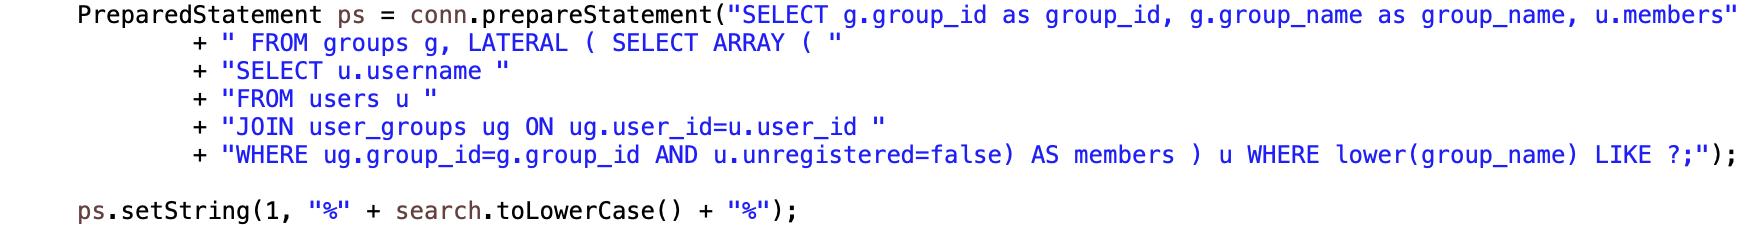
\includegraphics[width=\linewidth]{images/getSearchedGroupsCropped.png}}
  \caption{The getSearchedGroups method in DbConnection.java, the solution to a particularly difficult problem}
  \label{search-group}
\end{figure}


\textbf{Client} simply encapsulates a client user, and has fields such as username, id, email, publicKey, and a flag that states whether or not they are logged in.

\textbf{Group} simply encapsulates a group, and has fields such as group id, groupName, an array of group members and an array of members that left the group.

\textbf{ClientManager} is a singleton class that contains a HashMap to keep track of clients and specify which are online. As it follows the singleton design pattern, only one instance of this class can exist, so any time it is called on we can be sure that it is kept consistent and there will be no concurrency issues. The ClientManager is used by both ServerMain and DbConnection to determine when a client is online. ServerMain adds a client to the ClientManager when they Login, and removes them when the client closes the connection. DbConnection uses it to check whether a client is online or not when returning lists of clients. 

\textbf{ChatMessage} encapsulates a chat message, and has fields such as time sent, and username of the sender and recipient. 


\subsection{Database}

The Team Zero Server Database was implemented using PostgreSql and consists of 6 tables, as seen in figure \ref{db-schema} below.

\begin{figure}[H]
  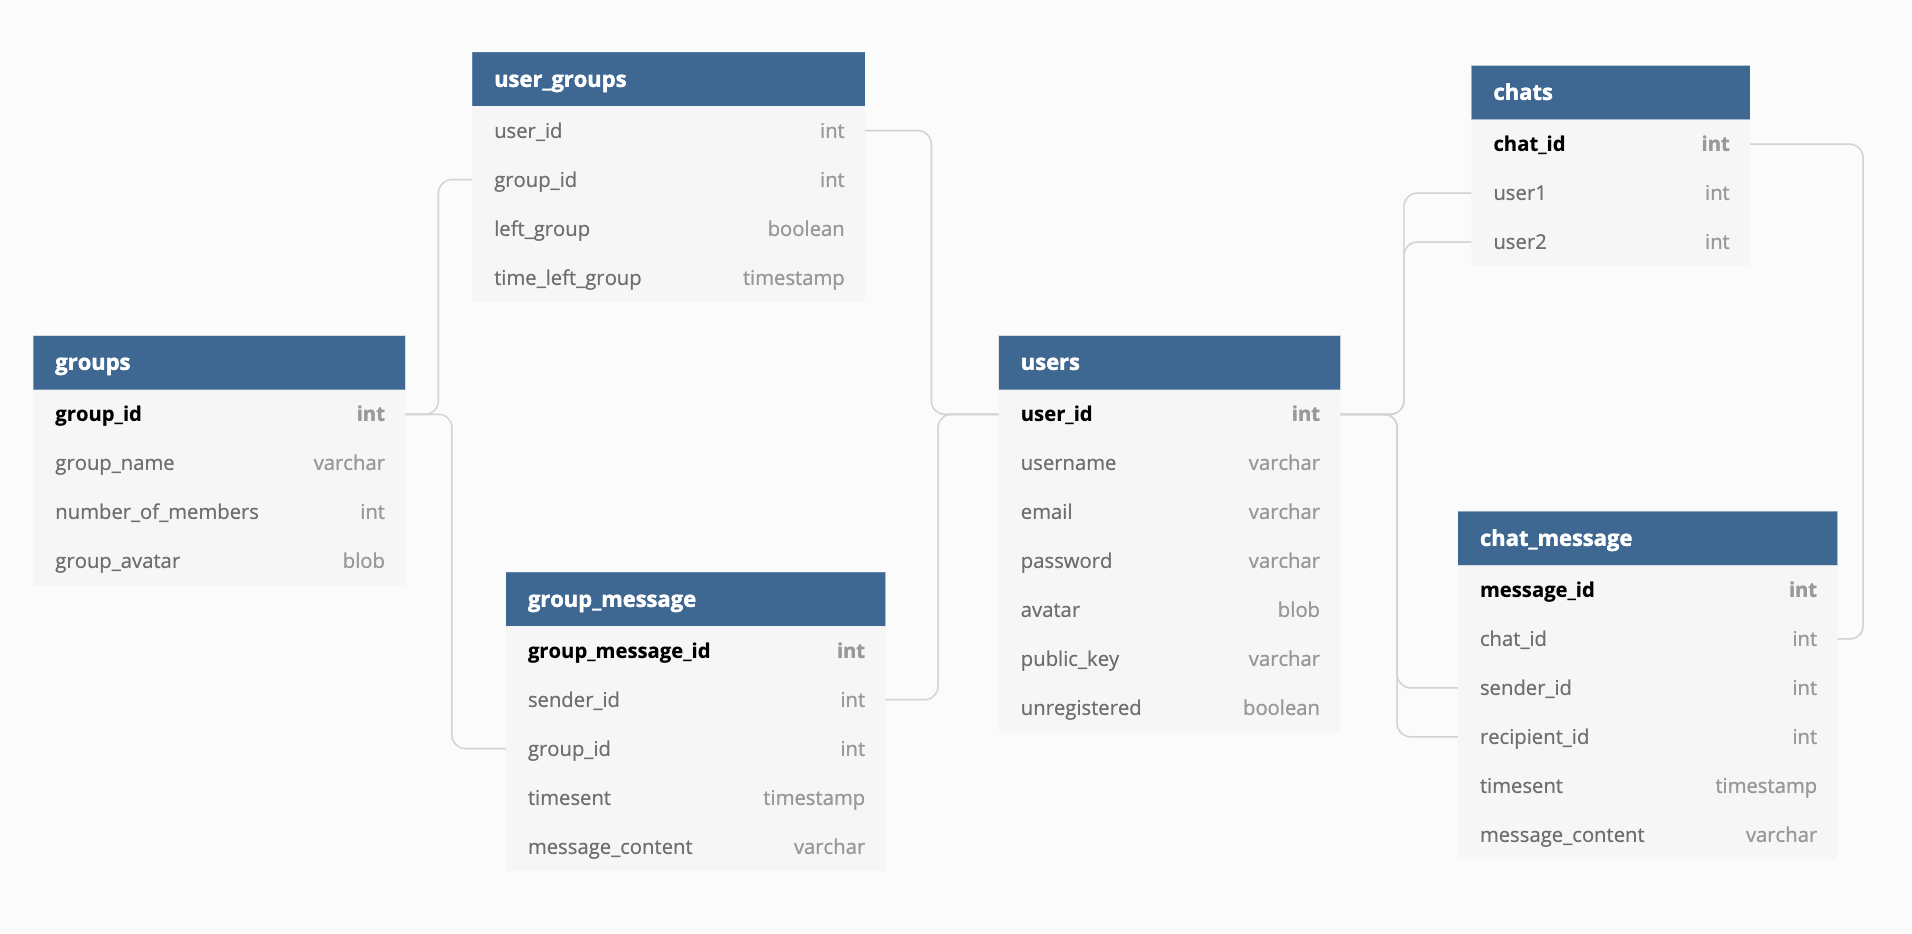
\includegraphics[width=\linewidth]{images/db.png}
  \caption{The Team Zero Server Database schema}
  \label{db-schema}
\end{figure}

A ``user" in the Team Zero Database is the same as a ``client" in Team Zero Server. This difference in terminology was agreed on due to the slight nuances in meaning - the database is referring to the individuals using the system, and the server is referring to the devices connected at the moment in time (even though they are one and the same at that moment in time).

Although the schema for the database was determined prior to implementation, there was generally not much need for change once implementation started. There was one main issue that required change, which was that once a user had sent any chat messages, their \verb|user_id| would become a required foreign key constraint, and the user would no longer be able to be deleted if they wished to unregister. This caused a problem once messaging functionality was implemented, as unregister tests began failing due to the database being unable to delete the user entry. We solved this issue by deciding to add an \verb|unregistered| flag to the \verb|users| table, setting it to true only if a user requests to unregister, and only including users with \verb|unregistered=false| entries in other queries. This same situation applied to group members leaving a group chat as well.


\subsection{Deployment to Heroku}

The database was deployed to Heroku, a cloud platform, to allow all group members to access and use it for testing purposes at any time. The data within the database can be viewed using the Pg Admin 4 software, which was also essential to our testing efforts.

We initially planned to also deploy the Team Zero Server application to Heroku as well, but unfortunately came across difficulties and decided to prioritise time on implementation, as local servers could be run on any machine for testing. 


\subsection{Server Interface for Client Communication (The API)}

\subsubsection{Requests accepted by Server}
\label{requestsToServer}


\begin{table}[H]
        \centering
        \small
        \setlength\tabcolsep{5pt}
\scriptsize
\begin{tabular}{ |c|c|c| } 
 \hline
 \textbf{Request type} & \textbf{Parameter} & \textbf{Parameter} \\
 \textbf{name} & \textbf{Name} & \textbf{description} \\
 \hline
 REGISTER & \verb|username| & User's username to register  \\ 
 & \verb|password| & Password associated with the username
 \\  &\verb|email|& User's email address
 \\  &\verb|picture|& User's profile picture
 \\  &\verb|publicKey|& User's public encryption Key
 \\  
  \hline
  LOGIN & \verb|username| & Username to login with  \\
  &\verb|password|& Password associated with username\\ 
  \hline
 TEXT & \verb|fromUsername| & Username of user sending the text message  \\ 
   & \verb|toUsername| & Username of intended recipient user
  \\  & \verb|message| & The text message \\ 
  \hline
 GETALLCONTACTS &  &   \\ 
  \hline
 SEARCHCONTACTS & \verb|search| & The search query \\ 
  \hline
 EDIT & \verb|username| & Username of editing user  \\ 
 &\verb|newPicture|& New profile picture to update \\
 &\verb|publicKey|& New public encryption key to update \\  
  \hline
 GETCHATHISTORY & \verb|myUsername| & Username of requesting user  \\ 
 &\verb|theirUsername|& Username of contact to get chat history of \\
 &\verb|historyDays|& how many days (int) of chat history to get \\  
  \hline
 UNREGISTER & \verb|username| & Unregistering user's username  \\ 
  &\verb|password|& Password associated with username \\ 
 \hline
 GETPUBLICKEY & \verb|username| & Username of the user whose public key is requested \\ 
  \hline
 CREATEGROUP & \verb|username| & Username of user creating the group  \\ 
   & \verb|groupName| & Name to give to group \\ 
  \hline
 JOINGROUP & \verb|username| & Username of user joining the group  \\ 
   & \verb|groupName| & Name of group to join \\ 
  \hline
 GROUPTEXT & \verb|sender| & Username of user sending the message \\ 
 &\verb|groupName|& Name of group to send the message to \\
 &\verb|messsage|& The text message \\  
  \hline
 GETALLGROUPS &  &   \\ 
  \hline
 SEARCHGROUPS & \verb|search| & The search query  \\ 
 \hline
  GETGROUPHISTORY & \verb|myUsername| & Username of requesting user \\ 
 &\verb|groupName|& Name of group to to get the history of \\
 &\verb|historyDays|& how many days (int) of chat history to get \\  
  \hline
  GETALLUSERGROUPS & \verb|myUsername| & Username of requesting user \\ 
  \hline
  REMOVEGROUPMEMBER & \verb|myUsername| & Username of requesting user \\ 
 &\verb|groupName|& Name of group to exit \\  
  \hline
  SEARCHUSERSNOTINGROUP & \verb|search| & The search query \\ 
 &\verb|groupName|& Name of group to search for users in \\  
  \hline
\end{tabular}
\end{table}



Notes:
\begin{itemize} 
\item UNREGISTER does not delete a user, it only sets a flag in the database. This allows their chat messages to remain in other users' chat histories. However, their username and email cannot be used again for a new registration.
\item GETCHATHISTORY will return the chat history in order with most recent history first.
\item Once a user creates a group, they automatically join the group - there is no need to separately do a JOINGROUP request.
\item GETGROUPHISTORY will return the group chat history in order with most recent history first and if the user requesting the history is not part of the group, it will return the group chat history till the time they were part of the group.
\item REMOVEGROUPMEMBER does not delete a user from a group, it only sets a flag in the database and sets the time of exit. This allows their group chat messages to remain in other users' group chat histories and allows this user to view the chat history of the group they left till the time they were inside the group. However, they can't be added again to the group.
\item The server keeps a HashMap object of any TEXT or GROUPTEXT messages awaiting sending (to clients who are not currently connected) and will send them on connection. In the case of several messages to be sent on connection, each message is sent separately with 10ms of sleep in between to avoid overloading the clients and causing them to crash (this 10ms of sleep was introduced after some integration tests which caused clients to crash).
\end{itemize}

%See Appendix \ref{requestToServerAppendix} for how these requests should be used with the given parameters in a JSON string, for the server to accept them.

\subsubsection{Replies returned from Server}
\label{repliesFromServer}



\begin{table}[H]
        \centering
        \small
        \setlength\tabcolsep{5pt}
\scriptsize
\begin{tabular}{ |c|c|c| } 
 \hline
 \textbf{Reply} & \textbf{Parameter} & \textbf{Parameter} \\
 \textbf{From} & \textbf{Name} & \textbf{description} \\
 \hline
 LOGIN & \verb|reply| & states which reply type it is and whether it was a success\\ 
 REGISTER &  &   or failure  \\ 
 EDIT & \verb|message| & an optional status message  \\ 
 UNREGISTER &  &  \\  
 CREATEGROUP &  &  \\  
 JOINGROUP &  &  \\  
  \hline
  TEXT & \verb|sender| & Username of text message sender  \\
  &\verb|recipient|& Username of text message recipient \\ 
  & \verb|message| & Text message   \\ 
   & \verb|timestamp| & Time received at server in format yyyy-MM-dd HH:mm:ss \\ 
  \hline
 GETALLCONTACTS & \verb|reply| &  states whether it was a success or failure \\ 
  & \verb|contacts| &  A JSON array of User information \\ 
  \hline
 SEARCHCONTACTS & \verb|reply| &  states whether it was a success or failure \\ 
  & \verb|contacts| &  A JSON array of User information \\ 
  \hline
 GETCHATHISTORY & \verb|reply| &  states whether it was a success or failure \\ 
  & \verb|messages| &  A JSON array of message information \\ 
  \hline
 GETPUBLICKEY & \verb|reply| &  states whether it was a success or failure \\ 
  & \verb|username| &  username of the associated public key \\ 
  & \verb|publicKey| &  Public encryption key in base 64 format \\ 
  \hline
 GETALLGROUPS & \verb|reply| &  states whether it was a success or failure \\ 
  & \verb|contacts| &  A JSON array of Group information (name and members) \\ 
  \hline
 SEARCHGROUPS & \verb|reply| &  states whether it was a success or failure \\ 
  & \verb|contacts| &  A JSON array of Group information (name and members) \\ 
  \hline
  GETALLUSERGROUPS & \verb|reply| &  states whether it was a success or failure \\ 
  & \verb|contacts| &  A JSON array of Group information (name and members) \\ 
  \hline
  GROUPTEXT & \verb|sender| & Username of text message sender  \\
  &\verb|groupName|& Name of group message was sent to \\ 
  & \verb|message| & Text message   \\ 
   & \verb|timestamp| & Time received at server in format yyyy-MM-dd HH:mm:ss \\ 
  \hline
  GETGROUPHISTORY & \verb|reply| &  states whether it was a success or failure \\ 
  & \verb|messages| &  A JSON array of message information \\ 
  \hline
  REMOVEGROUPMEMBER & \verb|reply| &  states whether it was a success or failure \\ 
  & \verb|messages| &  An optional status message \\ 
  \hline
  SEARCHUSERSNOTINGROUP & \verb|reply| &  states whether it was a success or failure \\ 
  & \verb|messages| &  A JSON array of User information \\ 
  \hline
 
\end{tabular}
\end{table}


%See Appendix \ref{dataReturnedFromServerAppendix} for how these requests should be used with the given parameters in a JSON string, for the server to accept them.



\subsubsection{Possible error replies from Server}
\label{api}

\begin{table}[H]
        \centering
        \small
        \setlength\tabcolsep{5pt}
\scriptsize
\begin{tabular}{ |c |c|c| } 
 \hline
 \textbf{Possible error reply from} & \textbf{Situation} & \textbf{Possible response message } \\
 \hline
 REGISTER & User uses an existing username & ``Username already exists"  \\ 
 & User uses an existing email & ``Email already exists"
 \\  
  \hline
  LOGIN & incorrect username or password & ``Cannot authenticate user. \\
  &&Check login details."  \\
   \hline
 TEXT & User did not log in & ``Sender is not logged in"   \\ 
  \hline
 GETALLCONTACTS & User did not log in & ``User is not logged in" \\ 
  \hline
 SEARCHCONTACTS & User did not log in  & ``User is not logged in" \\ 
  \hline
 EDIT & User did not log in & ``User is not logged in" \\
  \hline
 GETCHATHISTORY  & User did not log in & ``User is not logged in"  \\
  \hline
 UNREGISTER  & User did not log in & ``User is not logged in"  \\ 
 \hline
 GETPUBLICKEY & Bad username given & ``No user found with given username"  \\ 
 \hline
 CREATEGROUP & User did not log in & ``User is not logged in" \\
 & User gives an existing group name & ``Groupname already exists"  \\ 
 \hline
 JOINGROUP& User did not log in & ``User is not logged in" \\
  & User gives a nonexistant group name & ``Group name does not exist"  \\ 
 \hline
 GETALLGROUPS& User did not log in & ``User is not logged in" \\
 \hline
 SEARCHGROUPS & User did not log in & ``User is not logged in" \\ 
 \hline
 GROUPTEXT & User did not log in & ``User is not logged in" \\
 & Either a username or group name is bad & ``No such group with member in it"  \\ 
 \hline
 GETGROUPHISTORY  & User did not log in & ``User is not logged in"  \\
  \hline
  GETALLUSERGROUPS& User did not log in & ``User is not logged in" \\
 \hline
 REMOVEGROUPMEMBER  & User did not log in & ``User is not logged in"  \\
  \hline
  SEARCHUSERSNOTINGROUP& User did not log in & ``User is not logged in" \\
 \hline
 Other &  Unsupported request name given & ``unrecognised type"  \\ 
 & Unparsable string (Not JSON compliant) & ``bad JSON Format"\\ \hline
 Database issue & internal bug & SQLException message\\ 
  \hline
\end{tabular}
\end{table}


\subsection{Testing with a Test Client}

As the server implementation involves many interconnected parts and requires a websocket connection to access ServerMain, the ServerTesterClient was implemented to test individual functionalities to be as close to unit testing as possible. The client is a text based Java application which connects to the server using the websocket protocols, and sends JSON requests to perform tests as required. The output of this client can be analysed and checked against the server's logs to see if the messages received are as expected. 

Each request and reply outlined in section \ref{api} above was tested in various scenarios using the test client, including tests that expected error replies based on situations such as trying to create a new group and giving an existing group name. Testing was done throughout implementation, during and after each feature implemented, and included checking for potential bugs in previously implemented features as well. 

Figure \ref{clientTest} below shows a sample output from the ServerTesterClient.


\begin{figure}[H]
  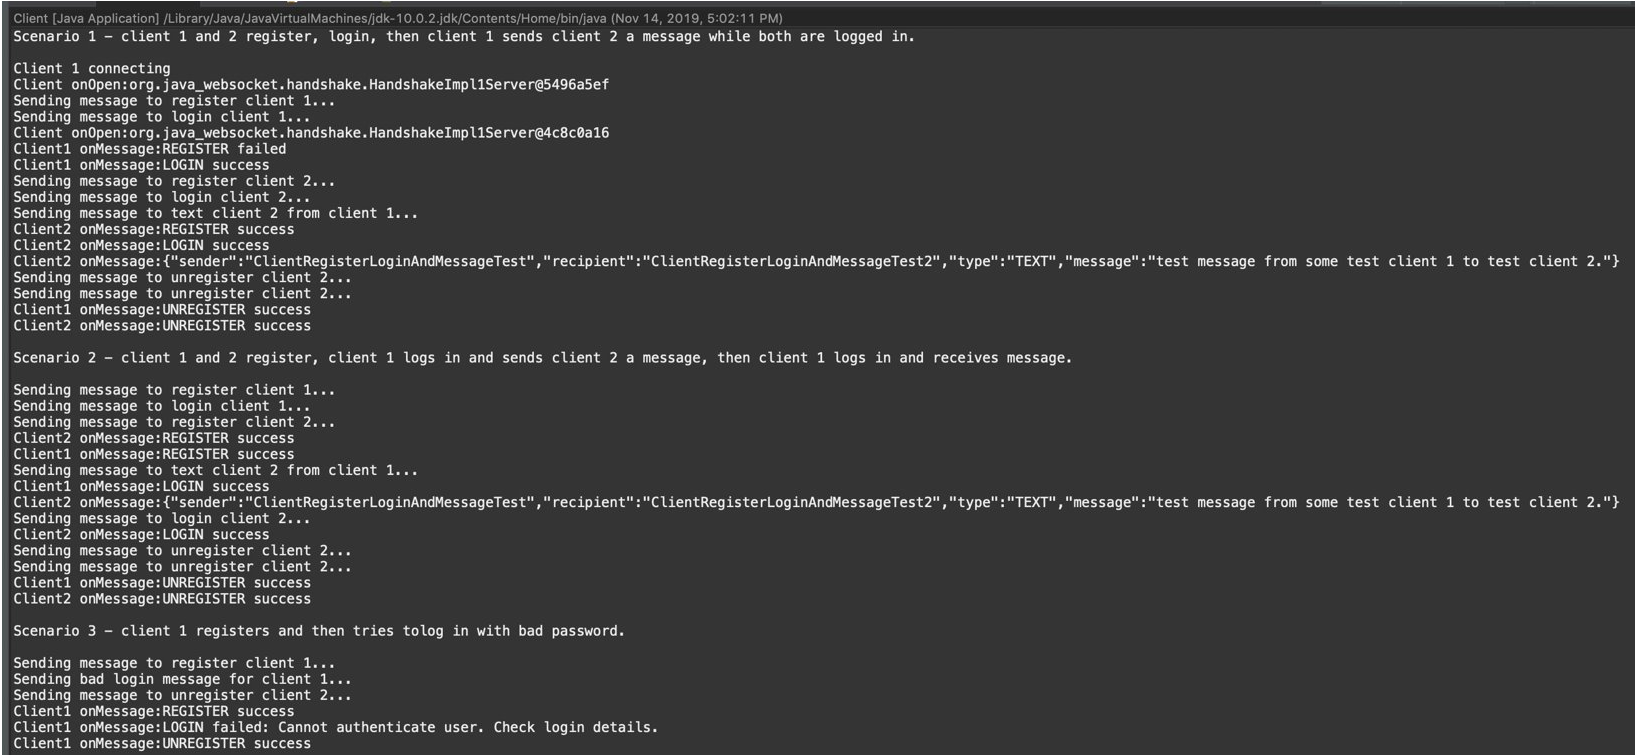
\includegraphics[width=\linewidth]{images/clientTest.png}
  \caption{Sample output from the ServerTesterClient}
  \label{clientTest}
\end{figure}
